\documentclass{standalone}
\usepackage{tikz}
\usepackage{lmodern}
\usepackage[T1]{fontenc}
\usepackage{graphicx}
\begin{document}
\begin{tabular}{ccc}

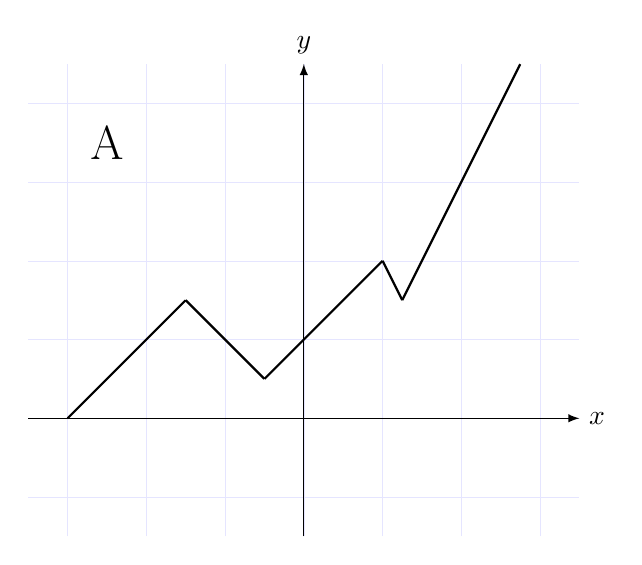
\begin{tikzpicture}[domain=-2:2,samples=100,scale=1.0,>=latex]
\tikzset{bgrid/.style={help lines,color=blue!10,very thin}}

\draw[bgrid] (-3.5,-1.5) grid (3.5,4.5);

\draw[->, color=black] (-3.5,0) -- (3.5,0) node[right] {$x$};
\draw[->, color=black] (0,-1.5) -- (0,4.5) node[above] {$y$};

\draw[thick,color=black,domain=-3:-1.5,smooth]
plot (\x,{\x+3});

\draw[thick,color=black,domain=-1.5:-0.5,smooth]
plot (\x,{-\x});

\draw[thick,color=black,domain=-0.5:1,smooth]
plot (\x,{\x+1});	

\draw[thick,color=black,domain=1:1.25,smooth]
plot (\x,{-2*\x+4});

\draw[thick,color=black,domain=1.25:2.75,smooth]
plot (\x,{2*\x-1});

\draw(-2.5,3.5) node {\LARGE A };
\end{tikzpicture}
 & 
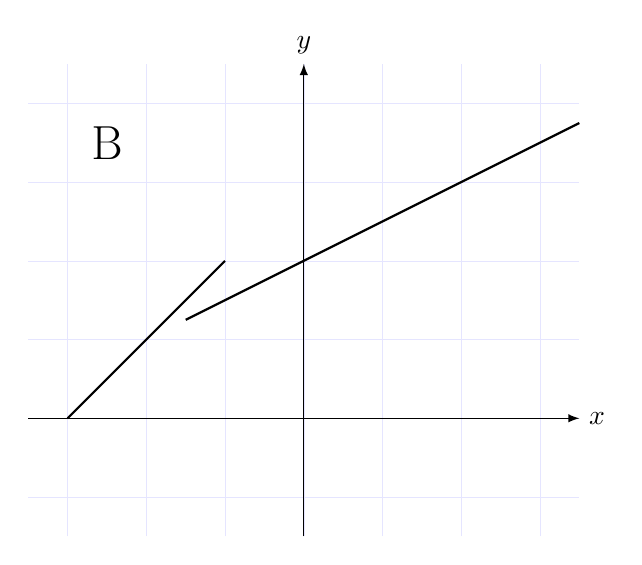
\begin{tikzpicture}[domain=-2:2,samples=100,scale=1.0,>=latex]
\tikzset{bgrid/.style={help lines,color=blue!10,very thin}}

\draw[bgrid] (-3.5,-1.5) grid (3.5,4.5);

\draw[->, color=black] (-3.5,0) -- (3.5,0) node[right] {$x$};
\draw[->, color=black] (0,-1.5) -- (0,4.5) node[above] {$y$};

\draw[thick,color=black,domain=-3:-1,smooth]
plot (\x,{\x+3});

\draw[thick,color=black,domain=-1.5:3.5,smooth]
plot (\x,{0.5*\x + 2});

\draw(-2.5,3.5) node {\LARGE B };
\end{tikzpicture}
 
& 

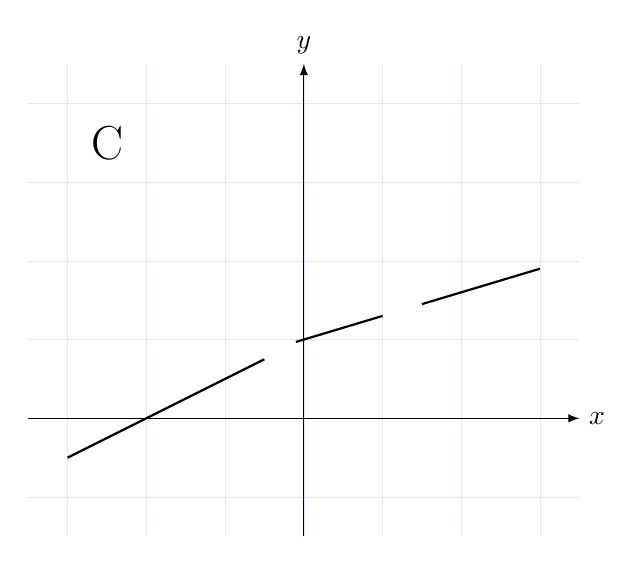
\begin{tikzpicture}[domain=-2:2,samples=100,scale=1.0,>=latex]
\tikzset{bgrid/.style={help lines,color=blue!10,very thin}}

\draw[bgrid] (-3.5,-1.5) grid (3.5,4.5);

\draw[->, color=black] (-3.5,0) -- (3.5,0) node[right] {$x$};
\draw[->, color=black] (0,-1.5) -- (0,4.5) node[above] {$y$};

\draw[thick,color=black,domain=-3:-0.5,smooth]
plot (\x,{0.5*\x + 1});

\draw[thick,color=black,domain=-0.1:1,smooth]
plot (\x,{0.3*\x+1});
\draw[thick,color=black,domain=1.5:3,smooth]
plot (\x,{0.3*\x+1});

\draw(-2.5,3.5) node {\LARGE C };
\end{tikzpicture}

\\

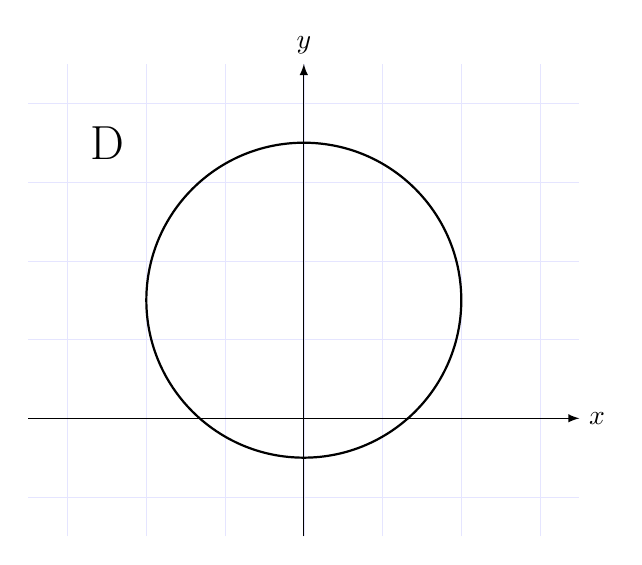
\begin{tikzpicture}[domain=-2:2,samples=100,scale=1.0,>=latex]
\tikzset{bgrid/.style={help lines,color=blue!10,very thin}}

\draw[bgrid] (-3.5,-1.5) grid (3.5,4.5);

\draw[->, color=black] (-3.5,0) -- (3.5,0) node[right] {$x$};
\draw[->, color=black] (0,-1.5) -- (0,4.5) node[above] {$y$};

\draw[thick,color=black,domain=-3:-1,smooth] (0,1.5) circle(2cm);
\draw(-2.5,3.5) node {\LARGE D };
\end{tikzpicture}

& 

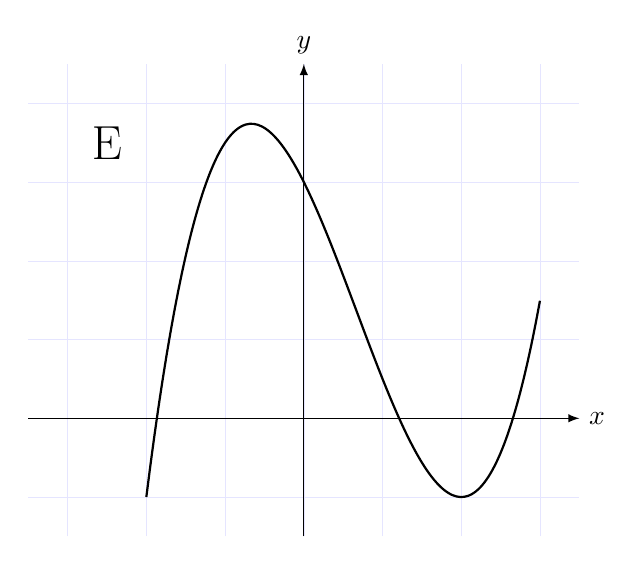
\begin{tikzpicture}[domain=-2:2,samples=100,scale=1.0,>=latex]
\tikzset{bgrid/.style={help lines,color=blue!10,very thin}}

\draw[bgrid] (-3.5,-1.5) grid (3.5,4.5);

\draw[->, color=black] (-3.5,0) -- (3.5,0) node[right] {$x$};
\draw[->, color=black] (0,-1.5) -- (0,4.5) node[above] {$y$};

\draw[thick,color=black,domain=-2:3,smooth]
plot (\x,{0.5*\x^3 -\x*\x -2*\x + 3});
\draw(-2.5,3.5) node {\LARGE E };
\end{tikzpicture}

& 

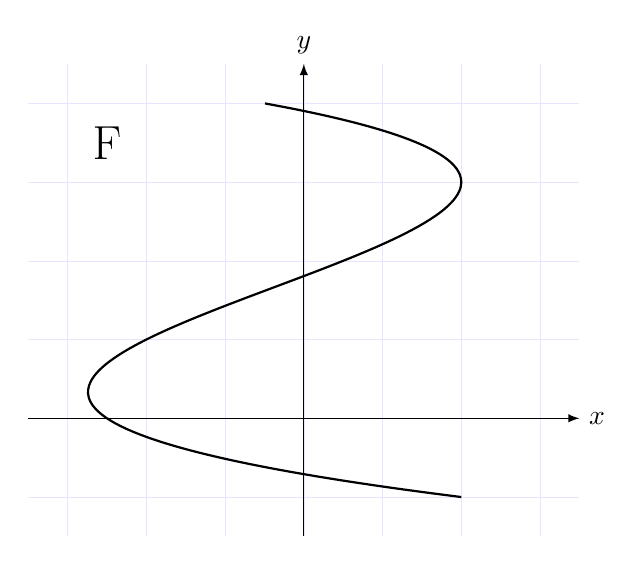
\begin{tikzpicture}[domain=-2:2,samples=100,scale=1.0,>=latex]
\tikzset{bgrid/.style={help lines,color=blue!10,very thin}}

\draw[bgrid] (-3.5,-1.5) grid (3.5,4.5);

\draw[->, color=black] (-3.5,0) -- (3.5,0) node[right] {$x$};
\draw[->, color=black] (0,-1.5) -- (0,4.5) node[above] {$y$};

\draw[thick,color=black,domain=-2:3,smooth, rotate=90, xshift=1cm, yshift=-1cm]
plot (\x,{0.5*\x^3 -\x*\x -2*\x + 3});
\draw(-2.5,3.5) node {\LARGE F };
\end{tikzpicture}

\end{tabular}
\end{document}